\documentclass[12pt,a4paper]{article}

\usepackage{geometry}
\usepackage{graphicx}
\usepackage{ragged2e}
\usepackage{multicol}
\usepackage{multirow}
\usepackage{adjustbox}
\usepackage{xcolor}
\usepackage{enumitem}

\usepackage{listings}
\usepackage{xcolor}

\lstset{
  basicstyle=\ttfamily\normalfont\scriptsize,
  breakatwhitespace=true,         
  escapeinside={\%*}{*)},
  breakautoindent=true,
  breaklines=true,                 
  captionpos=b,                    
  keepspaces=false,                 
  showspaces=false,                
  showstringspaces=false,
  showtabs=false,                  
  frame=single,
  numbers=none,
  stepnumber=1,% the step between two line-numbers. If it's 1 each line will be numbered
  tabsize=2
}

% Bash
\lstdefinelanguage{Bash}{
  morekeywords={
    if,then,else,elif,fi,for,while,do,done,case,esac,export
  },
  sensitive=true,
  morecomment=[l]\#,
  morestring=[b]",
}

% C
\lstdefinelanguage{C}{
  morekeywords={
    auto,break,case,char,const,continue,default,do,double,else,
    enum,extern,for,if,int,long,register,return,switch,typedef,
    unsigned,void,volatile,while
  },
  sensitive=true,
  morecomment=[l]//,
  morecomment=[s]/* */ ,
  morestring=[b]",
}

% C++
\lstdefinelanguage{C++}{
  morekeywords={
    alignas,alignof,and,asm,auto,bitand,bitor,bool,break,case,
    class,compl,const,constexpr,continue,decltype,default,delete,
    do,double,else,enum,explicit,false,for,friend,goto,if,inline,
    int,long,mutable namespace,new noexcept,operator,private,
    protected,public,register,return,short,signed,sizeof,
    static,static_assert,static_cast,struct,switch,template,this,
    thread_local,throw,true,try,typedef,typeid,typename,union,
    unsigned,using,virtual,void,volatile,wchar_t,while
  },
  sensitive=true,
  morecomment=[l]//,
  morecomment=[s]/* */ ,
  morestring=[b]",
}

% Java
\lstdefinelanguage{Java}{
  morekeywords={
    abstract,assert,boolean,break,byte,case,catch,char,class,
    const,continue,default,do,double,else,enum,extends,final,
    finally,float, for,goto,if,implements,import,instanceof,int,
    interface,long,native,new, null,package,private,protected,
    public,return,short,static,strictfp, super,switch,
    synchronized,this,throw,throws,transient,true,try,void,
    volatile,while
  },
  sensitive=true,
  morestring=[b]",
}

% Go
\lstdefinelanguage{Go}{
  morekeywords={
    break,case,chan,const,continue,
    default,defer,else,fallthrough,
    for,function,goto,if,import,interface,
    map,package,range,return,select,struct,
    switch,type,var},
  sensitive=true,
  morecomment=[l]//,
  morecomment=[s]/* */ ,
  morestring=[b]",
}

% PHP
\lstdefinelanguage{PHP}{
  morekeywords={
    __halt_compiler,abstract,alias,arguments,break,case,class,
    clone,const,continue,declare,default,die,do,echo,else,elseif,
    empty,endswitch,eval,exit,extends,final,finally,for,foreach,
    function,global,goto,if,implements,include,include_once,
    instanceof,insteadof,interface,is,isset,list,namespace,
    print,private,protected,public,return,static,switch,throw,
    trait,try,unset,use,var,while,yield
  },
  sensitive=true,
  morecomment=[l]//,
  morecomment=[s]/* */ ,
  morestring=[b]",
}

% Javascript
\lstdefinelanguage{JavaScript}{
    morekeywords={abstract,arguments,await,boolean,break,byte,
    case,catch,class,const,continue,debugger,default,delete,do,
    double,else,enum,eval,export,extends,false,finally,for,function,
    global,if,implements,import,in,instanceof,int,let,match,namespace,
    NaN,private,protected,public,return,super,switch,throw,throws,true,
    try,typeof,var,void,yield
  },
  sensitive=true,
  morecomment=[l]//,
  morecomment=[s]/* */ ,
  morestring=[b]",
}



\geometry{margin=1cm}
\graphicspath { {./img/} }

\pagenumbering{gobble}
\date{}


\lstdefinelanguage{SQL}{
  keywords={
    select, from, where, group, by, order, asc, desc, and, or, sum, count,
    as, is, null, not, like, join, on, inner, left, right, outer, distinct,
    SELECT, FROM, WHERE, GROUP, BY, ORDER, ASC, DESC, AND, OR, SUM, COUNT,
    AS, IS, NULL, NOT, LIKE, JOIN, ON, INNER, LEFT, RIGHT, OUTER, DISTINCT
  },
  keywordstyle=\bfseries\color{blue}, % Keywords in bold blue
  identifierstyle=\color{black},     % Identifiers in black
  stringstyle=\color{teal},          % Strings in teal
  commentstyle=\itshape\color{gray}, % Comments in italic gray
  morecomment=[l][\itshape\color{gray}]{--}, % SQL-style comments with --
  morestring=[b]"                   % Double-quoted strings
  }

  % Define the lstlisting style to use for SQL
  \lstset{
    language=SQL,
    basicstyle=\ttfamily\footnotesize, % Basic font style for all text
    numbers=none,                      % Line numbers on the left
    stepnumber=0,                      % Numbering each line
    numbersep=4pt,                     % Space between number and text
    backgroundcolor=\color{white},     % Background color
    frame=single,                      % Box around the code
    captionpos=b,                      % Caption at the bottom
    breaklines=true,                   % Automatic line breaking
    breakatwhitespace=true,            % Break lines only at whitespace
    showspaces=false,                  % Don't show spaces
    showstringspaces=false,            % Don't show spaces in strings
    }

    \newcommand{\codeListing}[1] { \lstinputlisting{./code/soal#1.sql} }

    \begin{document}

    NAMA: Radinal Shidiq Saragih

    KELAS: IF C 2023 

    NPM: 5520123104

    \begin{enumerate}

      \item Jelaskan apa yang di maksud Relational Database Management 
        System dan sebutkan beberapa 5 contoh produk dan vendor dari
        Database Management System (DBMS)

        \begin{enumerate}

          \item \textbf{Pengertian RDMBS (RDMS)}

            RDBMS atau Relational Database Management
            System adalah sistem managemen basis data yang
            berdasarkan data relasional atau berbentuk tabel.
            Data dalam jenis DBMS ini dihubungkan dengan satu
            sama lain dengan menggunakan suatu primary key
            unik.

          \item \textbf{Contoh RDMS}

            \begin{itemize}

              \item MySQL
              \item PostgresSQL
              \item Microsoft SQL Server
              \item Oracle

            \end{itemize}


        \end{enumerate}

      \item Diketahui sebuah tabel dengan data yang tidak normal seperti berikut ini

        \begin{center}
          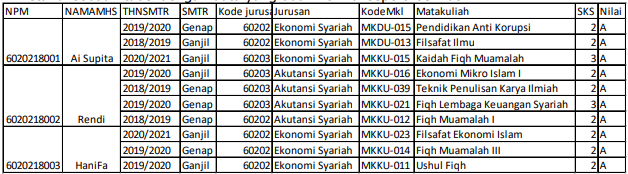
\includegraphics[scale=0.6]{TBSOAL2.png}
        \end{center}

        Buatlah dari data tabel di atas menjadi bentuk normal ke 3 (3NF)

        \begin{enumerate}

          \item Normal 1

            \begin{center}
              \begin{adjustbox}{width=\linewidth,center}
                \begin{tabular}{ |c|c|c|c|c|c|c|c|c|c| } 
                  \hline
                  NPM        & NAMAMHS   & THNSMTR   & SMTR    & kode jurusan & Jurusan         & KodeMkl & Matakuliah                     & SKS  & Nilai \\ \hline \hline
                  6020218001 & Ai Supita & 2019/2020 & Genap   & 60202        & Ekonomi Syariah & MKDU-15 & Pendidikan Anti Korupsi        & 2    & A     \\ \hline
                  6020218001 & Ai Supita & 2018/2020 & Ganjl   & 60202        & Ekonomi Syariah & MKDU-13 & Filsafat Ilmu           	     & 2    & A     \\ \hline
                  6020218001 & Ai Supita & 2020/2020 & Ganjil  & 60203        & Akutansi Syariah & MKKU-15 & Kaidah Fiqh Muamalah          & 2    & A     \\ \hline
                  6020218002 & Rendi     & 2019/2020 & Ganjil  & 60203        & Akutansi Syariah & MKDU-16 & Ekonomi Mikro Islam I         & 2    & A     \\ \hline
                  6020218002 & Rendi     & 2018/2020 & Genap   & 60203        & Akutansi Syariah & MKDU-39 & Teknik Penulisan Karya Ilmiah & 2    & A     \\ \hline
                  6020218002 & Rendi     & 2019/2020 & Genap   & 60203        & Akutansi Syariah & MKDU-21 & Fiqh Lembaga Keuangan Syariah & 3    & A     \\ \hline
                  6020218002 & Rendi     & 2018/2019 & Genap   & 60202        & Ekonomi Syariah  & MKDU-12 & Fiqh Muamalah I               & 2    & A     \\ \hline
                  6020218003 & Hanifa    & 2020/2021 & Ganjil  & 60202        & Ekonomi Syariah  & MKDU-23 & Filsafat Ekonomi Islam        & 2    & A     \\ \hline
                  6020218003 & Hanifa    & 2019/2020 & Genap   & 60202        & Ekonomi Syariah  & MKDU-14 & Fiqh Muamalah III             & 2    & A     \\ \hline
                  6020218003 & Hanifa    & 2019/2020 & Ganjil  & 60202        & Ekonomi Syariah  & MKDU-11 & Ishul Fiqh                    & 2    & A     \\ 
                  \hline
                \end{tabular}
              \end{adjustbox}
            \end{center}

          \item Normal 2

            \begin{adjustbox}{scale=0.5,center}
              \begin{tabular}{ |c|c|c|c|c|c| } 
                \hline
                \multicolumn{6}{|c|}{Tabel Nilai} \\ \hline
                NPM        & THNSMTR   & SMTR    & kode jurusan & KodeMkl & Nilai \\ \hline \hline
                6020218001 & 2019/2020 & Genap   & 60202        & MKDU-15 & A     \\ \hline
                6020218001 & 2018/2020 & Ganjl   & 60202        & MKDU-13 & A     \\ \hline
                6020218001 & 2020/2020 & Ganjil  & 60203        & MKDU-15 & A     \\ \hline
                6020218002 & 2019/2020 & Ganjil  & 60203        & MKDU-16 & A     \\ \hline
                6020218002 & 2018/2020 & Genap   & 60203        & MKDU-39 & A     \\ \hline
                6020218002 & 2019/2020 & Genap   & 60203        & MKDU-21 & A     \\ \hline
                6020218002 & 2018/2019 & Genap   & 60202        & MKDU-12 & A     \\ \hline
                6020218003 & 2020/2021 & Ganjil  & 60202        & MKDU-23 & A     \\ \hline
                6020218003 & 2019/2020 & Genap   & 60202        & MKDU-14 & A     \\ \hline
                6020218003 & 2019/2020 & Ganjil  & 60202        & MKDU-11 & A     \\ 
                \hline
              \end{tabular}
            \end{adjustbox}

            \begin{multicols}{3}
              \begin{adjustbox}{scale=0.5,center}
                \begin{tabular}{ |c|c|c| } 
                  \hline
                  \multicolumn{3}{|c|}{Tabel Matakuliah}  \\ \hline
                  KodeMkl & Matakuliah                    & SKS \\ \hline \hline
                  MKDU-11 & Ishul Fiqh                    & 2  \\ \hline                                    
                  MKDU-12 & Fiqh Muamalah I               & 2  \\ \hline                                    
                  MKDU-13 & Filsafat Ilmu           	    & 2  \\ \hline                                    
                  MKDU-14 & Fiqh Muamalah III             & 2  \\ \hline                                    
                  MKKU-15 & Kaidah Fiqh Muamalah          & 3  \\ \hline                                    
                  MKDU-15 & Pendidikan Anti Korupsi       & 2  \\ \hline                                    
                  MKDU-16 & Ekonomi Mikro Islam I         & 2  \\ \hline                                    
                  MKDU-21 & Fiqh Lembaga Keuangan Syariah & 3  \\ \hline                                    
                  MKDU-23 & Filsafat Ekonomi Islam        & 2  \\ \hline                                    
                  MKDU-39 & Teknik Penulisan Karya Ilmiah & 2  \\ \hline
                \end{tabular}
              \end{adjustbox}

              \begin{adjustbox}{scale=0.6,center}
                \begin{tabular}{ |c|c| } 
                  \hline
                  \multicolumn{2}{|c|}{Tabel Jurusan} \\ \hline
                  kode Jurusan  & Jurusan           \\ \hline \hline
                  60202         & Ekonomi Syariah   \\ \hline
                  60203         & Akutansi Syariah  \\ \hline
                \end{tabular}
              \end{adjustbox}

              \columnbreak

              \begin{adjustbox}{scale=0.6,center}
                \begin{tabular}{ |c|c| } 
                  \hline \multicolumn{2}{|c|}{Tabel Mahasiswa} \\ \hline
                  NPM        & NAMAMHS   \\ \hline \hline
                  6020218001 & Ai Supita \\ \hline
                  6020218002 & Rendi     \\ \hline
                  6020218003 & Hanifa    \\ \hline
                \end{tabular}
              \end{adjustbox}

            \end{multicols}

          \item Normal 3
            \begin{center}
            \end{center}


        \end{enumerate}

        \begin{adjustbox}{scale=0.5,center}
          \begin{tabular}{ |c|c|c|c|c| } 
            \hline
            \multicolumn{5}{|c|}{Tabel Nilai} \\ \hline
            NPM        & THNSMTR   & SMTR    &  KodeMkl & Nilai \\ \hline \hline
            6020218001 & 2019/2020 & Genap   &  MKDU-15 & A     \\ \hline
            6020218001 & 2018/2020 & Ganjl   &  MKDU-13 & A     \\ \hline
            6020218001 & 2020/2020 & Ganjil  &  MKDU-15 & A     \\ \hline
            6020218002 & 2019/2020 & Ganjil  &  MKDU-16 & A     \\ \hline
            6020218002 & 2018/2020 & Genap   &  MKDU-39 & A     \\ \hline
            6020218002 & 2019/2020 & Genap   &  MKDU-21 & A     \\ \hline
            6020218002 & 2018/2019 & Genap   &  MKDU-12 & A     \\ \hline
            6020218003 & 2020/2021 & Ganjil  &  MKDU-23 & A     \\ \hline
            6020218003 & 2019/2020 & Genap   &  MKDU-14 & A     \\ \hline
            6020218003 & 2019/2020 & Ganjil  &  MKDU-11 & A     \\ 
            \hline
          \end{tabular}
        \end{adjustbox}

        \begin{multicols}{3}
          \begin{adjustbox}{scale=0.5,center}
            \begin{tabular}{ |c|c| } 
              \hline
              \multicolumn{2}{|c|}{Tabel JurusanMatakuliah}  \\ \hline
              KodeMkl & kode jurusan \\ \hline \hline
              MKDU-11 & 60202        \\ \hline                                    
              MKDU-12 & 60202        \\ \hline                                    
              MKDU-13 & 60203        \\ \hline                                    
              MKDU-14 & 60203        \\ \hline                                    
              MKKU-15 & 60203        \\ \hline                                    
              MKDU-15 & 60203        \\ \hline                                    
              MKDU-16 & 60202        \\ \hline                                    
              MKDU-21 & 60202        \\ \hline                                    
              MKDU-23 & 60202        \\ \hline                                    
              MKDU-39 & 60202        \\ \hline
            \end{tabular}
          \end{adjustbox}

          \begin{adjustbox}{scale=0.5,center}
            \begin{tabular}{ |c|c|c| } 
              \hline
              \multicolumn{3}{|c|}{Tabel Matakuliah}  \\ \hline
              KodeMkl & Matakuliah                    & SKS \\ \hline \hline
              MKDU-11 & Ishul Fiqh                    & 2  \\ \hline                                    
              MKDU-12 & Fiqh Muamalah I               & 2  \\ \hline                                    
              MKDU-13 & Filsafat Ilmu           	    & 2  \\ \hline                                    
              MKDU-14 & Fiqh Muamalah III             & 2  \\ \hline                                    
              MKKU-15 & Kaidah Fiqh Muamalah          & 3  \\ \hline                                    
              MKDU-15 & Pendidikan Anti Korupsi       & 2  \\ \hline                                    
              MKDU-16 & Ekonomi Mikro Islam I         & 2  \\ \hline                                    
              MKDU-21 & Fiqh Lembaga Keuangan Syariah & 3  \\ \hline                                    
              MKDU-23 & Filsafat Ekonomi Islam        & 2  \\ \hline                                    
              MKDU-39 & Teknik Penulisan Karya Ilmiah & 2  \\ \hline
            \end{tabular}
          \end{adjustbox}

          \begin{adjustbox}{scale=0.6,center}
            \begin{tabular}{ |c|c| } 
              \hline
              \multicolumn{2}{|c|}{Tabel Jurusan} \\ \hline
              kode Jurusan  & Jurusan           \\ \hline \hline
              60202         & Ekonomi Syariah   \\ \hline
              60203         & Akutansi Syariah  \\ \hline
            \end{tabular}
          \end{adjustbox}

          \columnbreak

          \begin{adjustbox}{scale=0.6,center}
            \begin{tabular}{ |c|c| } 
              \hline \multicolumn{2}{|c|}{Tabel Mahasiswa} \\ \hline
              NPM        & NAMAMHS   \\ \hline \hline
              6020218001 & Ai Supita \\ \hline
              6020218002 & Rendi     \\ \hline
              6020218003 & Hanifa    \\ \hline
            \end{tabular}
          \end{adjustbox}

        \end{multicols}

      \item Diketahui sebuah tabel dengan data yang tidak normal seperti berikut ini

        \begin{center}
          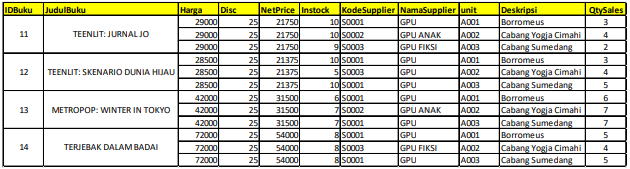
\includegraphics[scale=0.6]{TBSOAL3.png}
        \end{center}

        Buatlah dari data tabel di atas menjadi bentuk normal ke 3 (3NF)


        \begin{enumerate}

          \item Normal 1

            \begin{center}
              \begin{adjustbox}{scale=0.5,center}
                \begin{tabular}{ |c|c|c|c|c|c|c|c|c|c|c| } \hline
                  IDBuku & JudulBuku                    & Harga & Disc & NetPrice & Instock & KodeSupplier & NamaSupplier & Unit & Deskripsi           & QtySales \\ \hline
                  11     & TEENLIT:JURNAL IJO           & 29000 & 25   & 21750    & 10      & S0001        & GPU          & A001 & Borromeus           & 3        \\ \hline
                  11     & TEENLIT:JURNAL IJO           & 29000 & 25   & 21750    & 10      & S0002        & GPU ANAK     & A002 & Cabang Yogja Cimahi & 4        \\ \hline
                  11     & TEENLIT:JURNAL IJO           & 29000 & 25   & 21750    & 9       & S0003        & GPU FIKSI    & A003 & Cabang Sumedang     & 2        \\ \hline
                  12     & TEENLIT:SKENARIO DUNIA HIJAU & 28500 & 25   & 21375    & 10      & S0001        & GPU          & A001 & Borromeus           & 3        \\ \hline
                  12     & TEENLIT:SKENARIO DUNIA HIJAU & 28500 & 25   & 21375    & 5       & S0003        & GPU          & A002 & Cabang Yogja Cimahi & 4        \\ \hline
                  12     & TEENLIT:SKENARIO DUNIA HIJAU & 28500 & 25   & 21375    & 10      & S0001        & GPU          & A003 & Cabang Sumedang     & 5        \\ \hline
                  13     & TEENLIT:WINTER IN TOKYO      & 42000 & 25   & 31500    & 6       & S0001        & GPU          & A001 & Borromeus           & 6        \\ \hline
                  13     & TEENLIT:WINTER IN TOKYO      & 42000 & 25   & 31500    & 7       & S0002        & GPU ANAK     & A002 & Cabang Yogja Cimahi & 7        \\ \hline
                  13     & TEENLIT:WINTER IN TOKYO      & 42000 & 25   & 31500    & 7       & S0001        & GPU          & A003 & Cabang Sumedang     & 7        \\ \hline
                  14     & TEENLIT:TERJEBAK DALAM BADAI & 72000 & 25   & 54000    & 8       & S0001        & GPU          & A001 & Borromeus           & 5        \\ \hline
                  14     & TEENLIT:TERJEBAK DALAM BADAI & 72000 & 25   & 54000    & 8       & S0003        & GPU FIKSI    & A002 & Cabang Yogja Cimahi & 4        \\ \hline
                  14     & TEENLIT:TERJEBAK DALAM BADAI & 72000 & 25   & 54000    & 8       & S0001        & GPU          & A003 & Cabang Sumedang     & 5        \\ \hline
                \end{tabular}
              \end{adjustbox}
            \end{center}


          \item Normal 2

            \begin{adjustbox}{scale=0.6,center}
              \begin{tabular}{ |c|c|c|c|c| } 
                \hline \multicolumn{5}{|c|}{Tabel Buku} \\ \hline \hline
                IDBuku & JudulBuku                    & Harga & Disc & NetPrice \\ \hline
                11     & TEENLIT:JURNAL IJO           & 29000 & 25   & 21750    \\ \hline
                12     & TEENLIT:SKENARIO DUNIA HIJAU & 28500 & 25   & 21375    \\ \hline
                13     & TEENLIT:WINTER IN TOKYO      & 42000 & 25   & 31500    \\ \hline
                14     & TEENLIT:TERJEBAK DALAM BADAI & 72000 & 25   & 54000    \\ \hline
              \end{tabular}
            \end{adjustbox}

            \begin{center}
              \begin{adjustbox}{scale=0.5,center}
                \begin{tabular}{ |c|c|c|c|c|c|c|c|c| } \hline
                  IDBuku &  Disc & NetPrice & Instock & KodeSupplier & NamaSupplier & Unit & Deskripsi           & QtySales \\ \hline
                  11     &  25   & 21750    & 10      & S0001        & GPU          & A001 & Borromeus           & 3        \\ \hline
                  11     &  25   & 21750    & 10      & S0002        & GPU ANAK     & A002 & Cabang Yogja Cimahi & 4        \\ \hline
                  11     &  25   & 21750    & 9       & S0003        & GPU FIKSI    & A003 & Cabang Sumedang     & 2        \\ \hline
                  12     &  25   & 21375    & 10      & S0001        & GPU          & A001 & Borromeus           & 3        \\ \hline
                  12     &  25   & 21375    & 5       & S0003        & GPU          & A002 & Cabang Yogja Cimahi & 4        \\ \hline
                  12     &  25   & 21375    & 10      & S0001        & GPU          & A003 & Cabang Sumedang     & 5        \\ \hline
                  13     &  25   & 31500    & 6       & S0001        & GPU          & A001 & Borromeus           & 6        \\ \hline
                  13     &  25   & 31500    & 7       & S0002        & GPU ANAK     & A002 & Cabang Yogja Cimahi & 7        \\ \hline
                  13     &  25   & 31500    & 7       & S0001        & GPU          & A003 & Cabang Sumedang     & 7        \\ \hline
                  14     &  25   & 54000    & 8       & S0001        & GPU          & A001 & Borromeus           & 5        \\ \hline
                  14     &  25   & 54000    & 8       & S0003        & GPU FIKSI    & A002 & Cabang Yogja Cimahi & 4        \\ \hline
                  14     &  25   & 54000    & 8       & S0001        & GPU          & A003 & Cabang Sumedang     & 5        \\ \hline
                \end{tabular}
              \end{adjustbox}
            \end{center}

          \item Normal 3

            \begin{adjustbox}{scale=0.6,center}
              \begin{tabular}{ |c|c|c|c| } 
                \hline \multicolumn{4}{|c|}{Tabel Buku} \\ \hline \hline
                IDBuku & JudulBuku                    & Harga & NetPrice \\ \hline
                11     & TEENLIT:JURNAL IJO           & 29000 & 21750    \\ \hline
                12     & TEENLIT:SKENARIO DUNIA HIJAU & 28500 & 21375    \\ \hline
                13     & TEENLIT:WINTER IN TOKYO      & 42000 & 31500    \\ \hline
                14     & TEENLIT:TERJEBAK DALAM BADAI & 72000 & 54000    \\ \hline
              \end{tabular}
            \end{adjustbox}

            \begin{multicols}{3}

              \begin{adjustbox}{scale=0.6,center}
                \begin{tabular}{ |c|c| } 
                  \hline \multicolumn{2}{|c|}{Tabel Supplier} \\ \hline \hline
                  Kode Supplier & NamaSupplier   \\ \hline \hline
                  S0001         & GPU            \\ \hline
                  S0002         & GPU ANAK       \\ \hline
                  S0003         & GPU FIKSI      \\ \hline
                \end{tabular}
              \end{adjustbox}


              \begin{adjustbox}{scale=0.6,center}
                \begin{tabular}{ |c|c| } 
                  \hline \multicolumn{2}{|c|}{Tabel Unit} \\ \hline \hline
                  Unit & Deskripsi           \\ \hline
                  A001 & Borromeus           \\ \hline
                  A002 & Cabang Yogja Cimahi \\ \hline
                  A003 & Cabang Sumedang     \\ \hline
                \end{tabular}
              \end{adjustbox}

            \begin{center}
              \begin{adjustbox}{scale=0.5,center}
                \begin{tabular}{ |c|c|c|c|c|c|c| } \hline
                  IDBuku &  Disc & NetPrice & Instock & KodeSupplier & Unit & QtySales \\ \hline
                  11     &  25   & 21750    & 10      & S0001        & A001 & 3        \\ \hline
                  11     &  25   & 21750    & 10      & S0002        & A002 & 4        \\ \hline
                  11     &  25   & 21750    & 9       & S0003        & A003 & 2        \\ \hline
                  12     &  25   & 21375    & 10      & S0001        & A001 & 3        \\ \hline
                  12     &  25   & 21375    & 5       & S0003        & A002 & 4        \\ \hline
                  12     &  25   & 21375    & 10      & S0001        & A003 & 5        \\ \hline
                  13     &  25   & 31500    & 6       & S0001        & A001 & 6        \\ \hline
                  13     &  25   & 31500    & 7       & S0002        & A002 & 7        \\ \hline
                  13     &  25   & 31500    & 7       & S0001        & A003 & 7        \\ \hline
                  14     &  25   & 54000    & 8       & S0001        & A001 & 5        \\ \hline
                  14     &  25   & 54000    & 8       & S0003        & A002 & 4        \\ \hline
                  14     &  25   & 54000    & 8       & S0001        & A003 & 5        \\ \hline
                \end{tabular}
              \end{adjustbox}
            \end{center}

            \end{multicols}

        \end{enumerate}

      \item Perusahan yang bergerak di bidang pariwisata akan membuat system informasi
        pengelolaan VILA yang tersebar di wilayah cianjur dan puncak bogor. Dengan permintaan
        pelanggan harus melakukan login terhadap aplikasi dan memilih berbagai type Vila dan
        fasilitas vila yang ada. Kemudian pelanggan akan melakukan booking atas vila tersebut
        dengan menyertakan berapa jumlah penghuni villa dewasa dan anak anak. Perusahaan
        tersebut juga mempunyai karyawan yang harus login pada aplikasi/system tersebut sesuai
        dengan rolenya masing-masing. Selain itu juga dalam vila tersebut mempunyai restoran
        dengan berbagai macam menu makanan yang bisa di pesan baik di anter ke villa maupun
        pesan langsung ke restoran, dan pelanggan melakukan pembayaran atas pesanan makanan
        dengan pesanan vila, dari kasus ini buatlah
        \begin{center}
          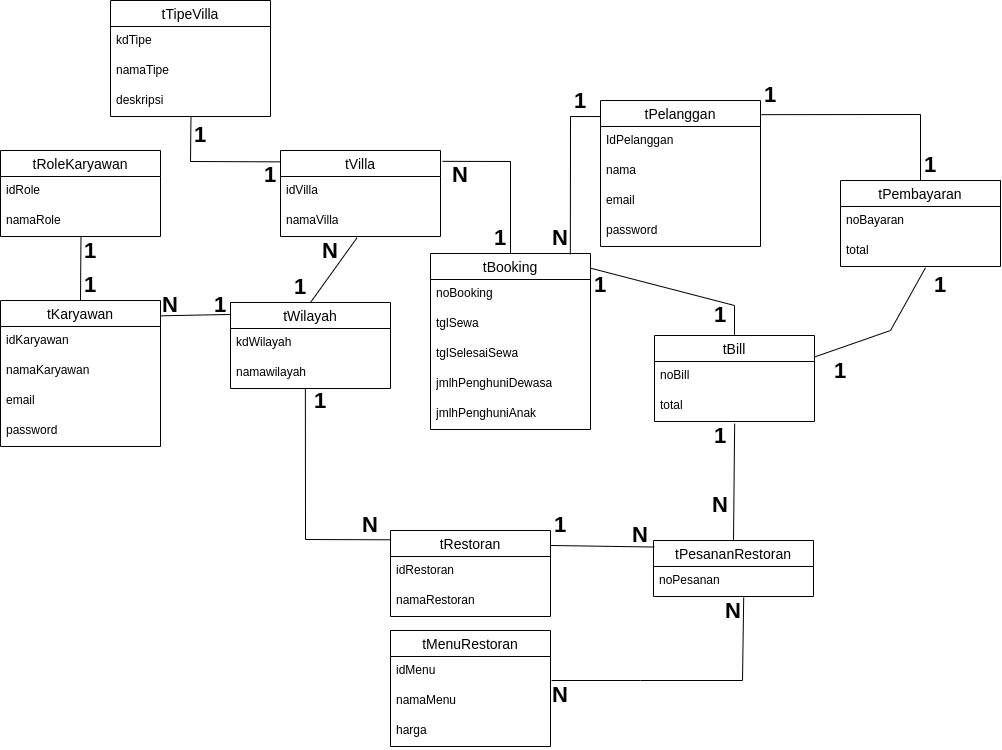
\includegraphics[scale=0.4]{ERDHOTEL.png}
        \end{center}

      \item Pada saat mendaftar menjadi anggota perpustakaan Fakultas, dicatatlah nama, nomor pokok
        mahasiswa dan alamat mahasiswa. Setelah itu mereka baru bisa meminjam buku diperpustakaan.
        Buku-buku yang dimiliki perpustakaan banyak sekali jumlahnya. Tiap judul buku memiliki data
        nomor buku atau nomor urut buku dengan judul yang sama, pengarang, penerbit, tahun terbit.
        Buku-buku tersebut di simpan di dalam rak dan di kelomokan berdasarkan katagory masingmasing. Jika terjadi telat pengembalian maka akan dikenakan biaya denda yang telah di tentukan,
        petugas bisa mengetahui data peminjaman dari fakultas dan prodi mana. Data dari kasus ini
        buatlah
        \begin{center}
          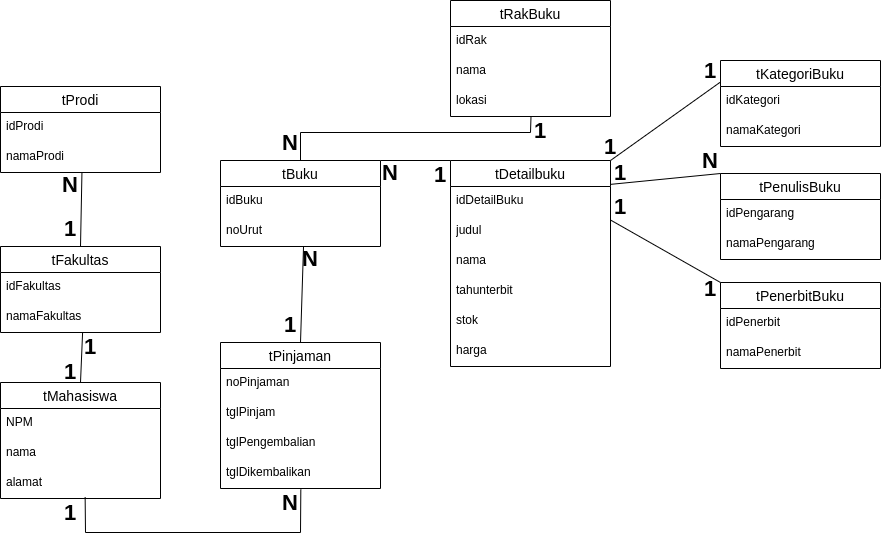
\includegraphics[scale=0.4]{ERDPERPUS.png}
        \end{center}

      \item Sebuah rumah sakit akang mengembangkan system informasi Radiologi, Dimana
        laboratoirm tersebut mempunyai karyawan yang akan di input ke system berdasarkan
        roulenya masing-masing. Pasien yang akan melakukan pemeriksaan melakukan
        pendafaran terlebih dahulu Tindakan apa yang akan di lakukan pemeriksaan, baik itu
        pasien rawat jalan maupun rawat inap. Setelah selesai pasien akan melakukan proses
        pembayaran berdasarkan jenis perawatan. Pasien yang melakukan rawat inap akan
        menempati ruangan dengan tipe kelas yang di pilih pasien. Pasien rawat inap akan di
        tangani oleh satu dokter dan 3 orang perawat.selain ada biaya Tindakan ada juga biaya
        proses mebaca hasil Tindakan yang dilakukan oleh dokter dengan nama biaya
        ekpertise(keahlian). Analisa dari soal cerita tersebut untuk di buat
        \begin{center}
          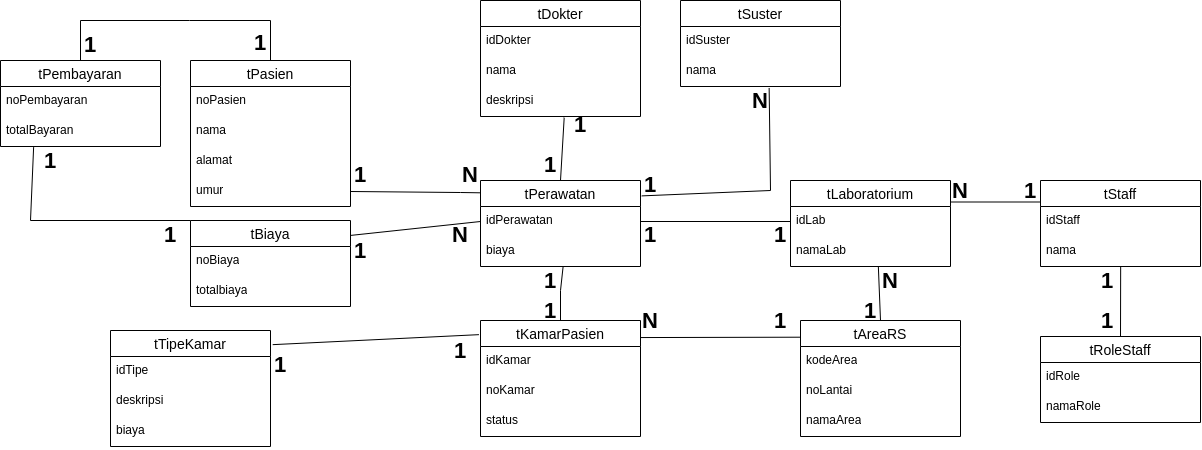
\includegraphics[scale=0.4]{ERDRS.png}
        \end{center}

      \newpage

      \item Apa yang anda ketahui tentang Trigers pada sebuah DBMS Jelaskan dan
        gambarkan prosesnya serta berikan contoh 

        \begin{enumerate}
          \item \textbf{Triggers After Insert}

            Trigger dijalankan setelah proses insert terjadi.

            Menambahkan data barang yang sudah terjual, maka otomatis jumlah
            pada table Tmasterbuku,TdetailMasterbuku, tdetailmasterbukuunit
            akan berkurang

            \lstinputlisting{./code/triggerAfterInsert.sql}

          \item \textbf{Triggers Before Insert}

            Trigger dijalankan sebelum proses insert terjadi.

            Memeriksa kode Subgroup pada Tabel
            tgroupcatagory, jika kodekatagory sudah ada maka akan muncul Pesan “Kode
            Group Sudah ada” dengan struktut table sebeperti berikut

            \begin{itemize}
              \item Table: tgroupcatagory
              \item Columns:
                \begin{itemize}
                  \item KodeCatagory varchar(5) PK
                  \item Nama varchar(100)
                \end{itemize}
            \end{itemize}

            \lstinputlisting{./code/triggerBeforeInsert.sql}

          \item \textbf{Triggers Before Update}

            Trigger dijalankan sebelum proses update terjadi.

            Pada Tabel tmasterbuku, fungsi triger ini untuk membuat history jika
            terjadi proses update data pada judul buku dengan proses memasukan
            data history ke sebauh table.

            \lstinputlisting{./code/triggerBeforeUpdate.sql}

        \end{enumerate}

      \newpage

      \item Perhatikan PDM dibawah ini

        \begin{center}
          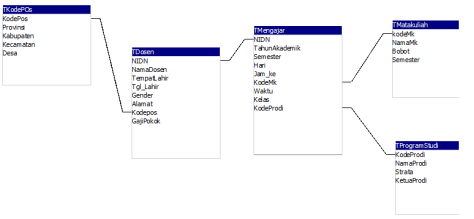
\includegraphics[scale=0.6]{TBSOAL8.png}
        \end{center}

        \begin{enumerate}

          \item Tampilkan NIDN,NamaDosen,TahunAkademik,semester, hari, jamke, 
            waktu,kelas,kodeprodi, namaprodi yang mengajar di hari senin

            \codeListing{1}

          \item Tampilkan NIDN,Namadosen, tempatlahir,tgllahir,gender,Alamat,
            desa,kecamatan,kabupaten,

            provinsi yang lahir di kota cianjur

            \codeListing{2}

          \item Tampilkan NIDN,NamaDosen,TahunAkademik,semester, hari, jamke,
            waktu,kelas,kodeprodi,

            namaprodi yang mengajar di hari kamis dengan
            program studi informatika

            \codeListing{3}

          \item Tampilkan NIDN,Namadosen, tempatlahir,
            tgllahir,gender,Alamat, desa,kecamatan,kabupaten,provinsi
            yang lahir di kota cianjur dan berjenis kelamin laki-laki

            \codeListing{4}

          \item Tampilkan NIDN,Namadosen, tempatlahir,tgllahir,gender, gajipokok,
            Alamat, desa,kecamatan,kabupaten,

            provinsi dengan gaji pokok di atas 5000000

            \codeListing{5}

        \end{enumerate}

    \end{enumerate}
  \end{document}
